% !TeX encoding = UTF-8
% !TeX spellcheck = pl_PL
\chapter{Tło teoretyczne}

\section{Mikrokontroler}
%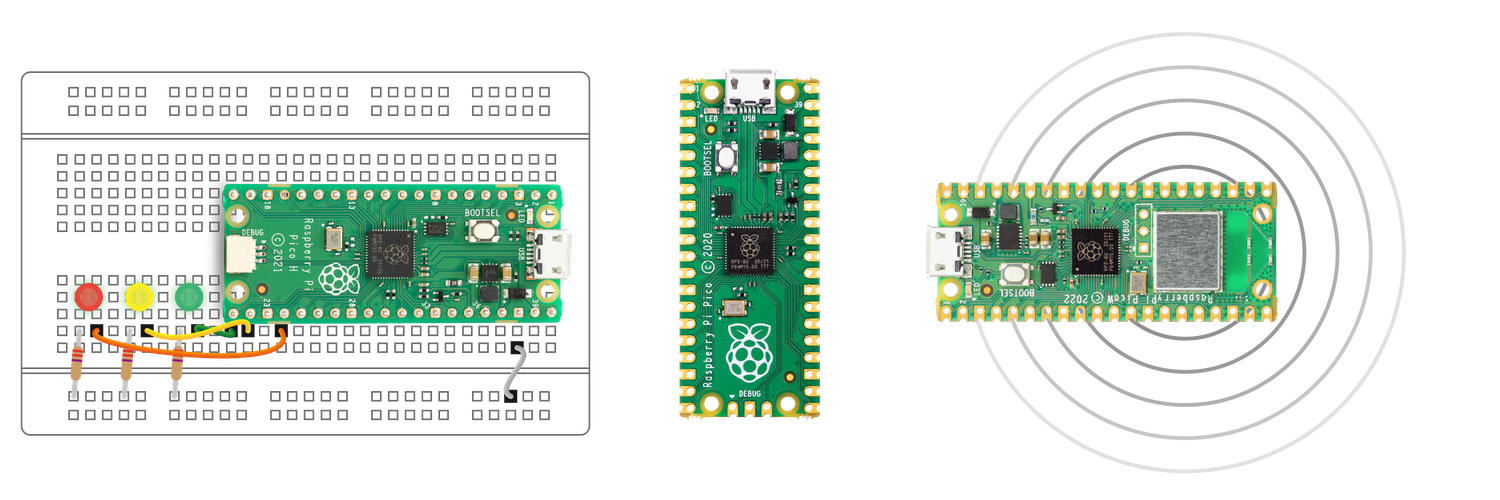
\includegraphics{rp2040.png} // zrobić fotkę mikrokontrolerowy
Mikrokontroler który wykorzystano to Raspberry Pico (RP2040)\cite{pico2024} w rozmiarze (z ang. form factor) 21 mm x 51 mm, z dwu-rdzeniowym procesorem Arm Cortex-M0+, z zegarem o maksymalnym taktowaniu 133 MHz. Ten "mini-komputer" posiada 264 kB SRAM-u i 2 MB pamięci QSPi, 26 wielofunkcyjnych pinów GPIO, włączając w to 3 wejścia analogowe.
Ponadto co jest szczególnie ważne w kwestii przyłączania zewnętrznych modułów mikrokontroler wyposażono w 2 UART, i co mniej ważne 2 SPI, 2 I2C i 16 kanałów PWM.
Do wgrywania programów udostępniono kontroler USB w wersji 1.1, z opcją hosta.
Obsługiwane napięcie wejściowe to od 1,8 V do 5,5 V DC.
Temperatura pracy to od -20 st. C do +85 st. C.
\section{Lora}
Jak podaje artykuł naukowy\cite{Augustin2016} LoRa to bezprzewodowy system telekomunikacyjny o dużym zasięgu, małej mocy i niskiej przepływności, promowany jako rozwiązanie infrastrukturalne dla Internetu rzeczy: urządzenia końcowe wykorzystują LoRa w pojedynczym przeskoku bezprzewodowym, aby komunikować się z bramą (bramkami), podłączonymi do Internetu, które działają jako przezroczyste mosty i przekazują wiadomości między tymi urządzeniami końcowymi a centralnym serwerem sieciowym. W artykule przedstawiono przegląd LoRa i dogłębną analizę jego funkcjonalnych komponentów.
W moim zastosowaniu nie będzie typowych bram, będą po prostu 2 urządzenia działające przy wykorzystaniu tego systemu.
LoRa jest ukierunkowana na zastosowania, w których urządzenia końcowe mają ograniczoną ilość energii (na przykład zasilane z baterii), w których urządzenia końcowe nie muszą przesyłać więcej niż kilka bajtów na raz i w których ruch danych może być inicjowany przez urządzenie końcowe lub przez podmiot zewnętrzny, który chce się z nim skomunikować. Charakter dalekiego zasięgu i niskiego poboru mocy LoRa sprawia, że jest to idealny kandydat do wykorzystania w tym projekcie.
LoRa zapewnia komunikację na duże odległości do 5 km w obszarach miejskich i do 15 km w obszarach wiejskich (w linii wzroku).
Protokół ten umożliwia tworzenie urządzeń, które na zasilaniu bateryjnym mogą działać nawet przez 10 lat.
\section{Bluetooth LE}
